% Shared standalone design for the editable figure reconstructions.
\documentclass[tikz,border=5pt,10pt]{standalone}
\usepackage[T1]{fontenc}
\usepackage[utf8]{inputenc}
\usepackage{newpxtext,newpxmath}
\usepackage[scaled=.94]{sourcesanspro}
\usepackage{pgfplots}
\pgfplotsset{compat=1.18}
\usetikzlibrary{arrows.meta,calc,positioning,decorations.pathreplacing,
  decorations.markings,patterns,matrix,shapes.geometric,fit,backgrounds,
  intersections,angles,quotes}
\definecolor{ink}{HTML}{203746}
\definecolor{accent}{HTML}{146C78}
\definecolor{muted}{HTML}{667780}
\definecolor{signalred}{HTML}{B94B44}
\color{ink}
\tikzset{>=Latex,line width=.8pt,
  every node/.style={font=\small},
  axis/.style={->,draw=muted,line width=.5pt},
  guide/.style={draw=muted,dashed,line width=.45pt},
  curve/.style={draw=accent,line width=1pt},
  marker/.style={circle,fill=accent,inner sep=1.5pt},
  labelbox/.style={fill=white,inner sep=2pt}}

\begin{document}
\begin{tikzpicture}[x=7cm,y=.36cm]
\draw[axis] (-.57,0)--(.62,0) node[right] {$k/N$};
\draw[axis] (0,-.1)--(0,10.8) node[above] {$-\lambda_k/N^2$};
\draw[signalred,dashed,line width=1pt,domain=-.5:.5,samples=151] plot (\x,{(2*pi*\x)^2});
\draw[curve,domain=-.5:.5,samples=151] plot (\x,{4*sin(180*\x)^2});
\foreach \x in {-.5,.5} {\draw[guide] (\x,0)--(\x,9.8696);\fill[signalred] (\x,9.8696) circle(1.6pt);\fill[accent] (\x,4) circle(1.6pt);}
\node[below] at (-.5,-.25) {$-\tfrac12$};\node[below] at (.5,-.25) {$\tfrac12$};\node[below left] at (0,0) {$0$};
\node[left] at (-.5,9.8696) {$\pi^2$};\node[left] at (-.5,4) {$4$};
\node[anchor=west,signalred] at (.67,8.7) {$(2\pi k/N)^2$};
\node[anchor=west,accent] at (.67,4.1) {$4\sin^2(\pi k/N)$};
\node[align=left] at (.12,-4.5) {continuum: $\lambda_k=-(2\pi k)^2$\\[3mm]discrete: $\lambda_k=-4N^2\sin^2(\pi k/N)$};
\end{tikzpicture}
\end{document}
